
\documentclass[handout]{beamer}
\usetheme{Singapore}
\usecolortheme[RGB={0, 32, 91}]{structure}  % Rice blue
\setbeamertemplate{navigation symbols}{\insertframenumber}

\usepackage{tabto}
\definecolor{ricegray}{rgb}{0.486, 0.494, 0.498}
\definecolor{dodgerblue}{rgb}{0.118, 0.565, 1.000}
\definecolor{darkorange}{rgb}{1.000, 0.549, 0.000}
\definecolor{forestgreen}{rgb}{0.133, 0.545, 0.133}

\title{The First Lesson of Sport Analytics}
\author{Dr. Scott Powers}
\date{\color{ricegray} Assistant Professor of Sport Analytics and of Statistics}

\begin{document}

  \begin{frame}
    \maketitle
    \vfill
    \hfill
\includegraphics[width = 4cm]{images/rice_logo.png}
  \end{frame}

  \begin{frame}{Play Ball!}
    \begin{columns}
      \begin{column}{0.6\columnwidth}
        \begin{enumerate}
          \item Scan the QR code\\
          ~\\
          \item Enter your batting average\\
          (from your piece of paper)\\
          ~\\
          \item Click {\bf Simulate!} (ONLY ONCE)\\
          ~\\
          \item How many hits did you get?
        \end{enumerate}
      \end{column}
      \begin{column}{0.4\columnwidth}
        \centering
        
\includegraphics[width=3cm]{images/qr_shinyapps.png}\\
        $\downarrow$\\
        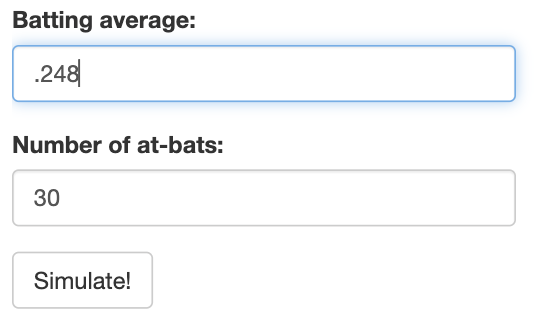
\includegraphics[width=\textwidth]{images/shinyapps.png}
      \end{column}
    \end{columns}
  \end{frame}

  \begin{frame}{You Be the Scout}
    \centering
    
\includegraphics[width=3cm]{images/qr_google.png}\\
    ~\\
    What is your guess of the number on the winner's piece of paper? The closest guess wins. Format your guess as a number: .XXX
  \end{frame}

  \begin{frame}
    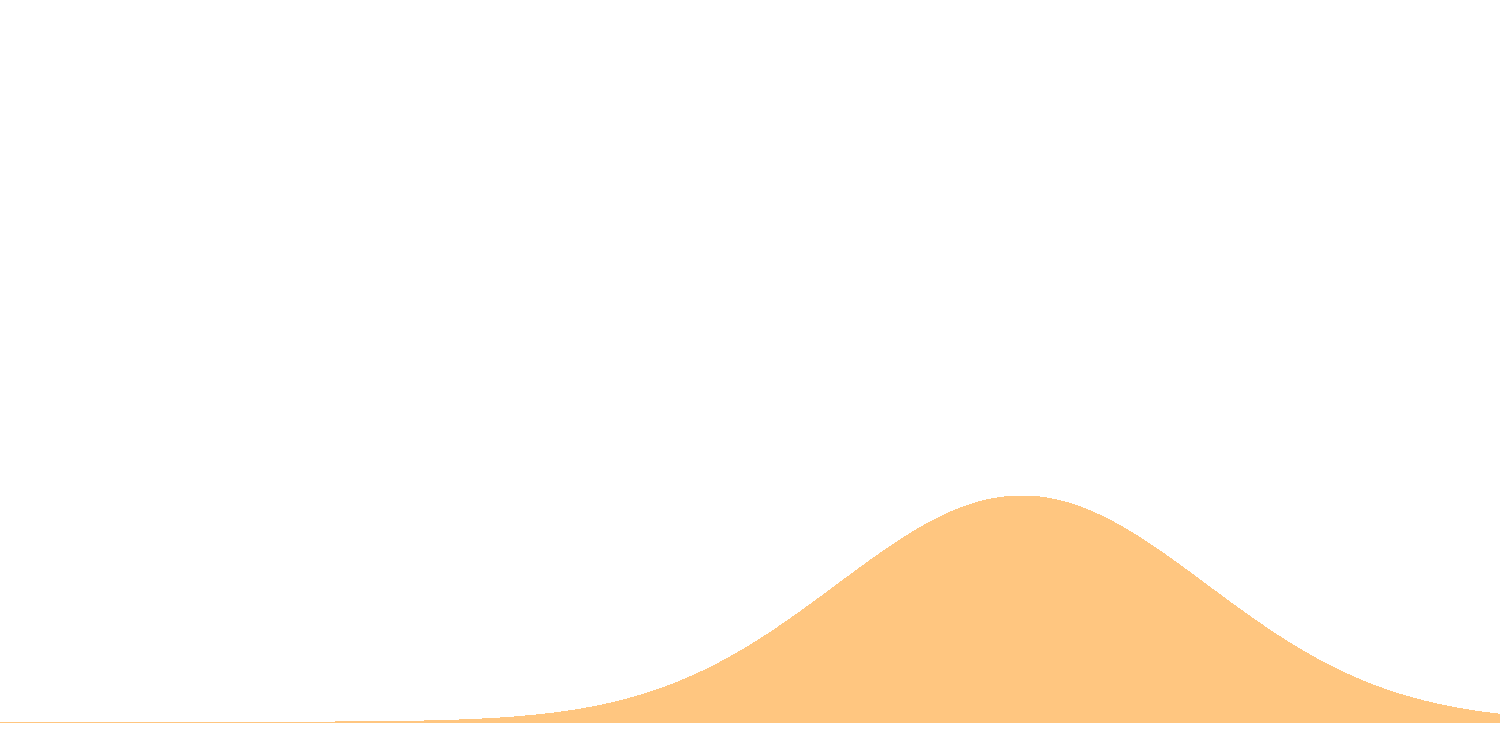
\includegraphics[width = \textwidth]{images/illustration_1.pdf}\\
    \tabto{73mm}$\uparrow$\\
    \tabto{73mm}$\hat p$
  \end{frame}

  \begin{frame}
    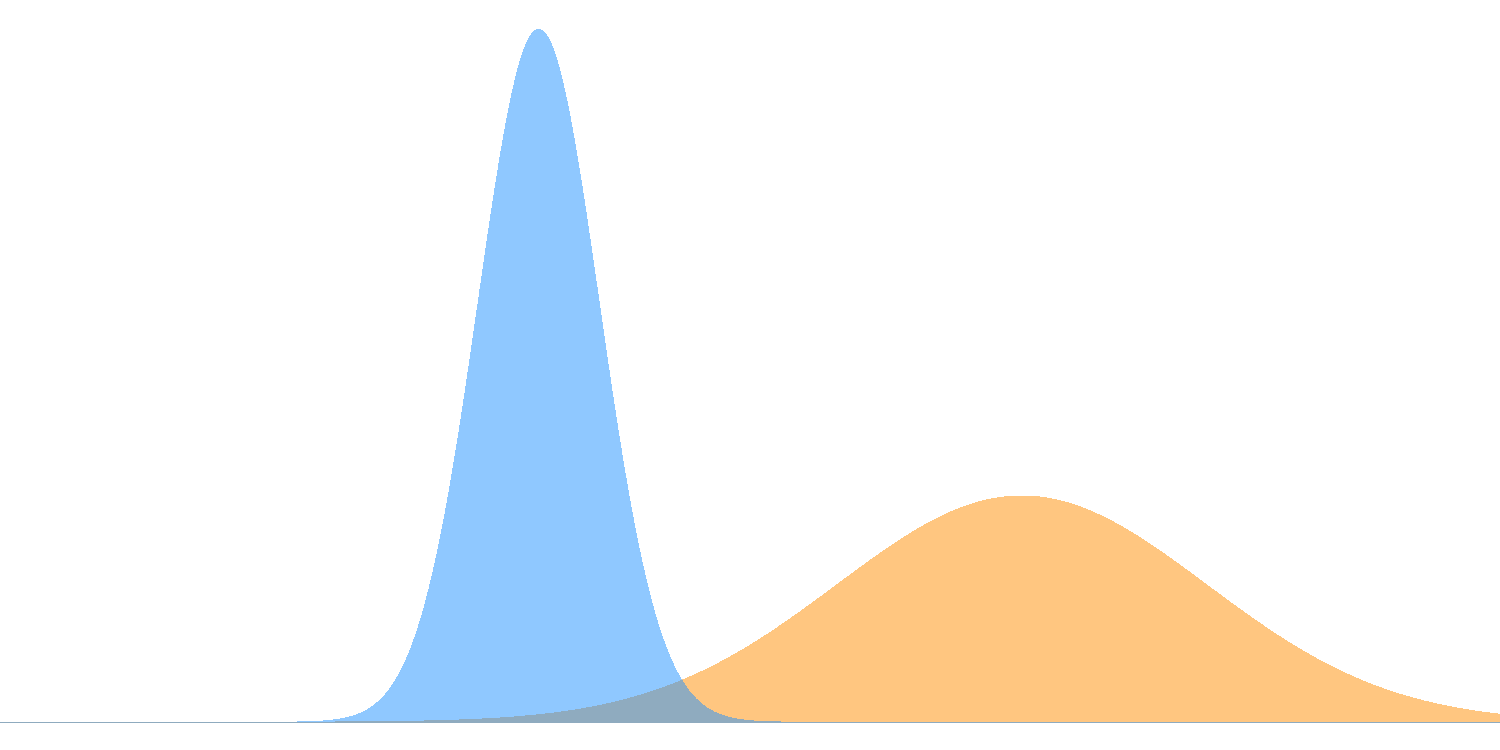
\includegraphics[width = \textwidth]{images/illustration_2.pdf}
    \tabto{38mm}$\uparrow$  \tabto{73mm}$\uparrow$\\
    \tabto{38mm}$\bar p$    \tabto{73mm}$\hat p$
  \end{frame}

  \begin{frame}
    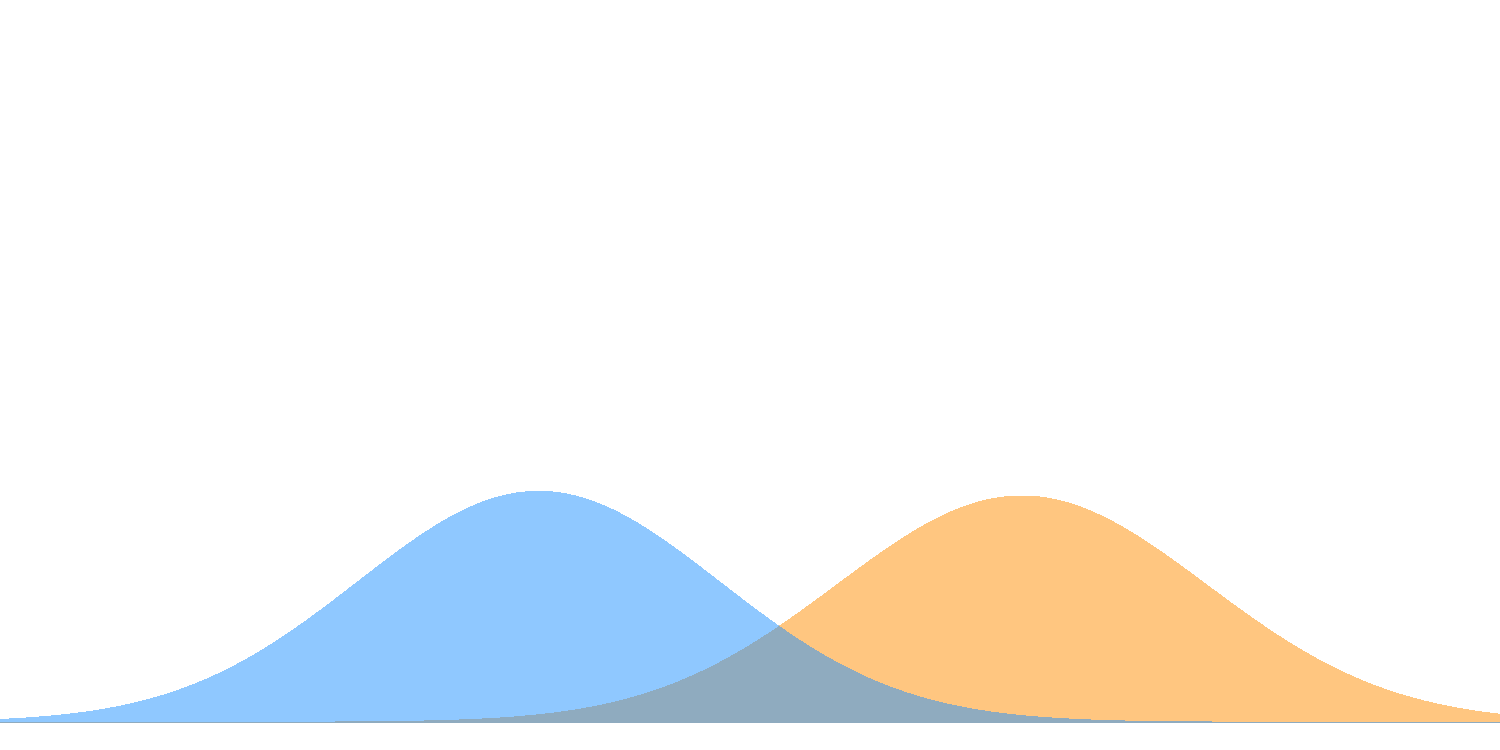
\includegraphics[width = \textwidth]{images/illustration_3.pdf}
    \tabto{38mm}$\uparrow$  \tabto{73mm}$\uparrow$\\
    \tabto{38mm}$\bar p$    \tabto{73mm}$\hat p$
  \end{frame}

  \begin{frame}
    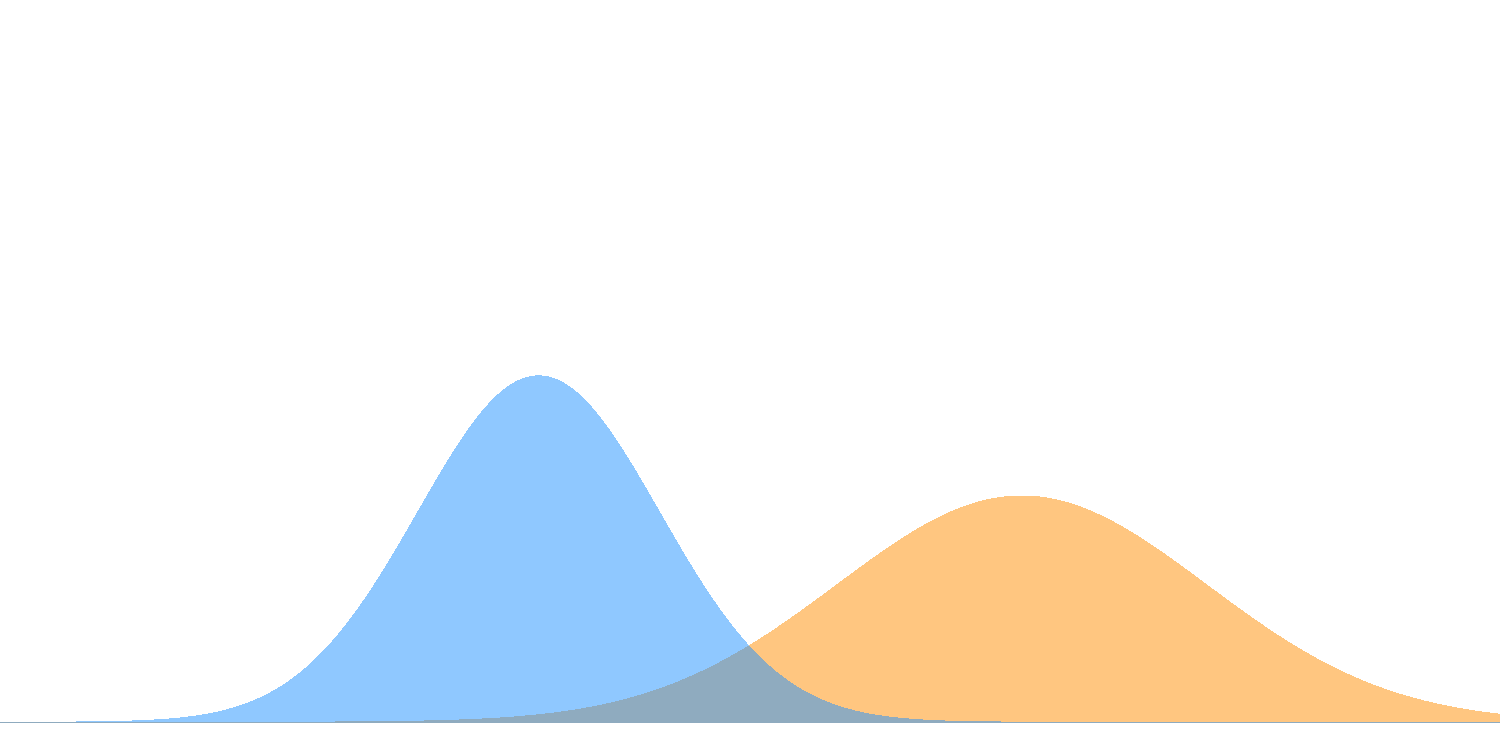
\includegraphics[width = \textwidth]{images/illustration_4.pdf}
    \tabto{38mm}$\uparrow$            \tabto{73mm}$\uparrow$\\
    \tabto{38mm}$\bar p \pm \sigma_T$ \tabto{73mm}$\hat p \pm \sigma_L$
  \end{frame}

  \begin{frame}
    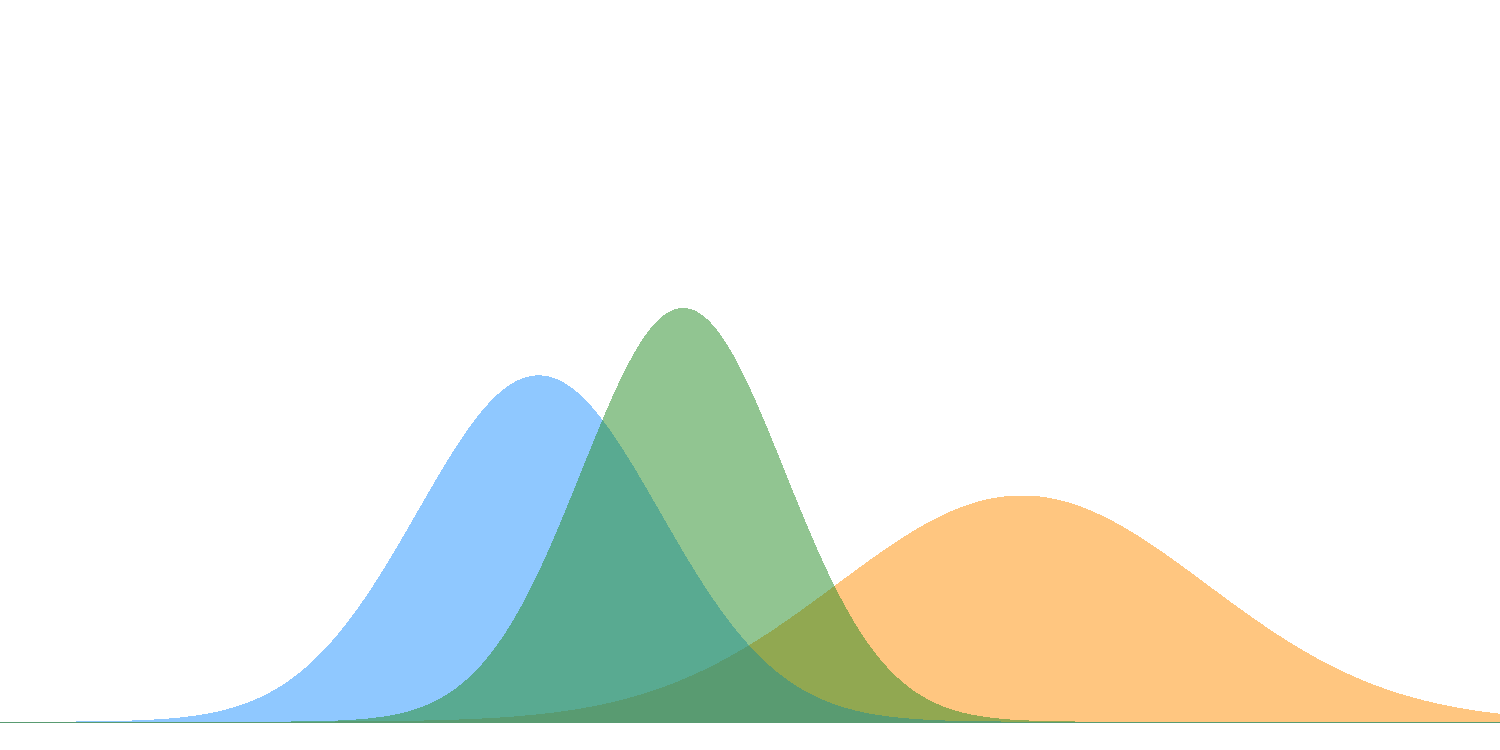
\includegraphics[width = \textwidth]{images/illustration_5.pdf}
    \tabto{38mm}$\uparrow$  \tabto{48mm}$\uparrow$  \tabto{73mm}$\uparrow$\\
    \tabto{38mm}$\bar p$    \tabto{48mm}$p^*$       \tabto{73mm}$\hat p$
  \end{frame}

  \begin{frame}{Regression to the Mean}
    $$p^* = \frac{\bar p {\color{dodgerblue}/ \sigma^2_T} + \hat p {\color{darkorange}/ \sigma^2_L}}{{\color{dodgerblue}1 / \sigma^2_T} + {\color{darkorange}1 / \sigma^2_L}}$$
    \vspace{1cm}\\
    \pause
    In our game: $\bar p = .250$, $\sigma_T = .020$ and $\sigma_L = \sqrt{.25 \cdot .75 / 30}$
    \tabto{45mm} $\Downarrow$ \tabto{69mm} $\Downarrow$
    \tabto{35mm} {\color{dodgerblue}$1 / \sigma_T^2 = 2500$} \tabto{60mm} {\color{darkorange}$1 / \sigma_L^2 = 160$}
    $$p^* = \frac{{\color{dodgerblue}2500} \cdot \bar p + {\color{darkorange} 160} \cdot \hat p}{{\color{dodgerblue}2500} + {\color{darkorange} 160}} = 94\% \cdot \bar p + 6\% \cdot \hat p$$
  \end{frame}

  \begin{frame}{The First Lesson of Sport Analytics}
    \begin{enumerate}
      \item Don't be fooled by noise.\\
      ~\\
      \pause
      \item (Bonus) In sport analytics we are (almost) always wrong.\\The objective to be a little less wrong than our competitors.
    \end{enumerate}
  \end{frame}

\end{document}
